\documentclass[10pt,aspectratio=43]{beamer}

%% Fonts
\usepackage{multicol}
\usepackage{mathabx}
\usepackage[scaled]{helvet}
\usepackage{lmodern}
\usepackage{eulervm}
\usepackage{natbib}
\usepackage{booktabs}
\usepackage{amsfonts}
%\usepackage{multicol}
%\usefonttheme[onlymath]{serif}
%\usefonttheme{professionalfonts}
\usefonttheme{structurebold}
\usepackage{bm}


%% Color & Theme
\definecolor{SUblue}{RGB}{0,0,180}
\usecolortheme[RGB={0,0,180}]{structure}
\usetheme{Boadilla}
\setbeamertemplate{navigation symbols}{}
\setbeamertemplate{itemize items}[circle]
\setbeamertemplate{enumerate items}[circle]
\setbeamerfont{title}{size=\large}
\setbeamerfont{frametitle}{size=\large}
\setbeamerfont{framesubtitle}{size=\large,shape =$\color{violet}{\looparrowdownright}~$}
\setbeamercolor{title}{fg=white, bg= SUblue!75!green}
\setbeamercolor{framesubtitle}{fg=violet}
%% \setlength{\leftmargini}{5pt}

\hypersetup{
  colorlinks=true,
  linkcolor=SUblue,
  citecolor=SUblue,
  urlcolor=SUblue}


\title[Covariate-Dependent Copula Modeling]{\textbf{Improving forecasting performance
    using \\covariate-dependent copula models}}



\author[Feng Li]{%\includegraphics[height=2cm]{cufelogo}\\
  \vspace{0.5cm}\textbf{Feng Li}\\
  \vspace{0.5cm} Joint with Yanfei Kang
  \\\vspace{0.3cm}\url{feng.li@cufe.edu.cn}\\\url{http://feng.li/}}

\institute[SAM.CUFE.EDU.CN]{\footnotesize{\textbf{School of Statistics and
      Mathematics\\ Central University of Finance and Economics}}}
\date{}

\begin{document}
%% Title page
\begin{frame}[plain]
  \addtocounter{framenumber}{-1}
  \titlepage
\end{frame}

\section*{Outline}
\begin{frame}
  \frametitle{Outline}
  \addtocounter{framenumber}{-1}
\tableofcontents
  \begin{itemize}
  \item[]   \vspace{2cm} \color{blue} \item [*] Feng Li's research is supported by National
    Natural Science Foundation of China.
  \end{itemize}

\end{frame}


% \begin{frame}
%   % \frametitle{Collaborators on the series of papers}
%   \begin{itemize}
%     % \item Yanfei Kang, Associate Professor, Beihang University, Beijing China.
%   % \item Zhuojing He, PhD student, Central University of Finance and Economics, Beijing
%   %   China.
%   % \item Anastasios Panagiotelis, Associate Professor, Monash University, Australia.


%   \end{itemize}


% \end{frame}


\section{Covariate-dependent copula models}


\begin{frame}
  \frametitle{What is a copula?}
  \begin{itemize}
  \item The word ``copula'' means \textbf{linking}.
  \item \textbf{Sklar's theorem}

    Let $H$ be a multi-dimensional distribution function with marginal
    distribution functions $F_1(x_1),...,F_m(x_m)$. Then there exists a
    function $C$ (\textbf{copula function}) such that
    \begin{equation*}
      \begin{split}
        H(x_1,...,x_m)= & C(F_1(x_1),...,F_m(x_m))\\
        =&C\left(\int_{-\infty}^{x_1}f(z_1)dz_1,...,\int_{-\infty}^{x_m}f(z_m)dz_m\right)=C(u_1,...,u_m).
      \end{split}
    \end{equation*}
    Furthermore, if $F_i(x_i)$ are continuous, then $C$ is unique, and the derivative $c(u_1,...,u_m)= \partial^m C(u_1,...,u_m)/(\partial u_1...
    \partial u_m)$ is the \textbf{copula density}.

  \end{itemize}
\end{frame}



\begin{frame}
  \frametitle{Covariate-dependent copula models}
  \framesubtitle{The Joe-Clayton copula example}
  \begin{itemize}
  \item The Joe-Clayton copula function \citep{joe1997multivariate}
    \[
    \begin{split}
      C(u,v,\theta,\delta)=&1-\left[1-\left\{\left(1-\bar u ^{\theta }\right)^{-\delta
          }+\left(1-\bar v ^{\theta }\right)^{-\delta }-1\right\}^{-1/\delta
        }\right]^{1/\theta }
    \end{split}
    \]
    where $\theta \geq 1$, $\delta > 0$, $\bar u = 1-u$, $\bar v = 1-v$ .

  \item Some properties:
    \begin{itemize}

    \item $\lambda_L=2^{-1/\delta}$ does not depend on $\lambda_U=2-2^{-1/\theta}$.
    \item  $\tau=1- 4\int _0^{\infty} s\times(\varphi'(s))^2ds$ is calculated via Laplace
      transform.

    \item A symmetric copula when $\lambda_L=\lambda_U$ is easily
      constructed \citep{patton2006modelling}.




    \end{itemize}
  \end{itemize}

\end{frame}

\begin{frame}[plain]
  % \frametitle{The covariate-contingent copula model}
  % \framesubtitle{The dependence and correlation of Joe-Clayton copula}
  \begin{figure}
    \centering
    \vspace{-0.35cm}
    \includegraphics[width=0.46\textwidth]{BB7_tau-lamba}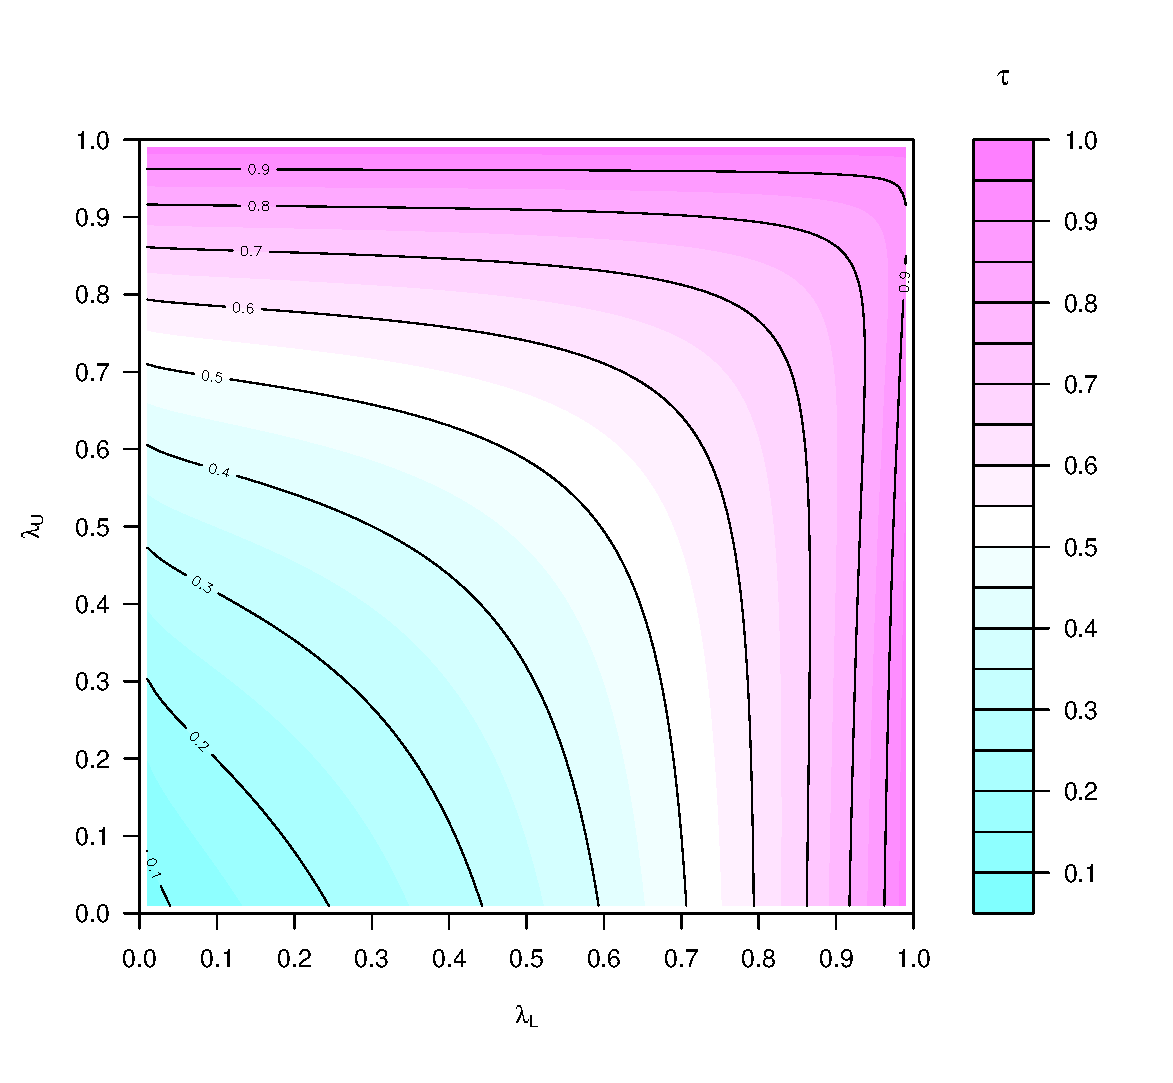
\includegraphics[width=0.56\textwidth]{tau-contour}\\
    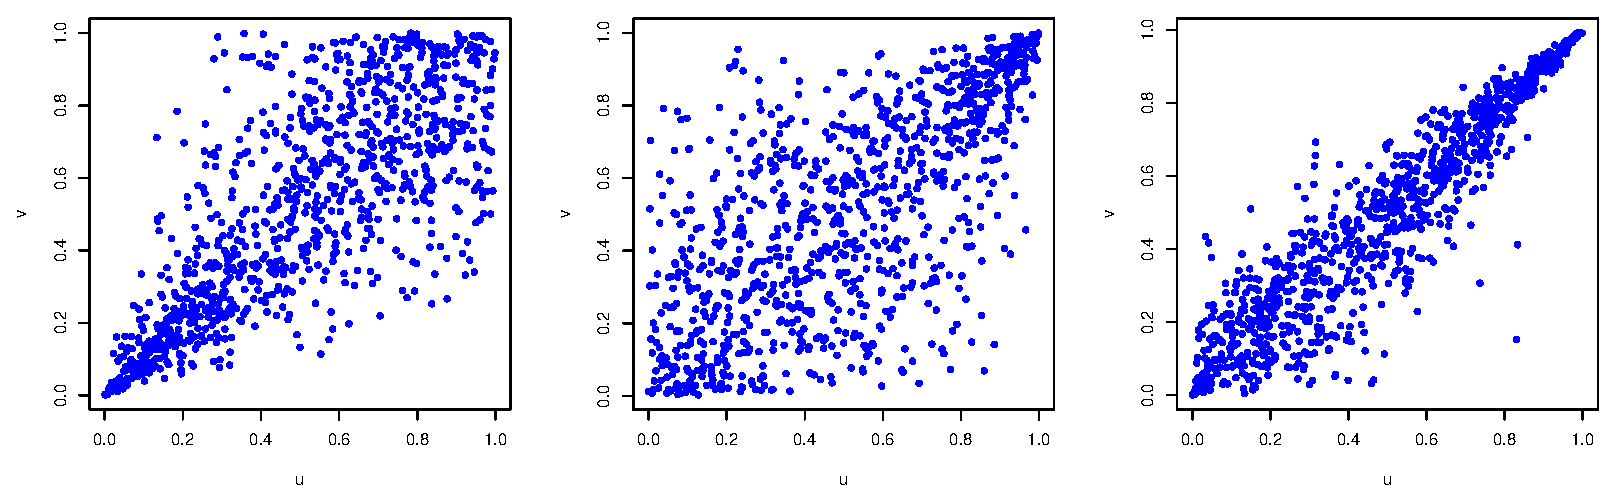
\includegraphics[width=\textwidth]{BB7Scatter}
  \end{figure}
\end{frame}


\begin{frame}
  \frametitle{Covariate-dependent copula models}
  \framesubtitle{The reparameterized copula model}
  \begin{itemize}

  % \item \textbf{The motivation} i) The interpretation of correlation and tail-dependence.
  %   ii) Dynamical modeling tail-dependence and correlation.

  \item \textbf{Reparametrization}: We reparameterize the copula as a function of
    tail-dependence and/or Kendall's tau $C(\bm{u},\lambda_L,\tau)$.

  \item \textbf{Link with covariates}: All copula features in the $k$:th and $l$:th margins can be connected with
    covariates
      \begin{align*}
        \tau_{kl}&=l_{\tau}^{-1}(\bm{X}_{kl}\bm{\beta}_{\tau}),\\
        \lambda_{kl}&=l_{\lambda}^{-1}(\bm{X}_{kl}\bm{\beta}_{\lambda})
      \end{align*}

    \item \textbf{Applicable Copulas}: Any copula can be equally well used with such
      reparameterization when there is closed form of tail-dependence and Kendall's
      $\tau$.

    \begin{itemize}
    \item \textbf{Archimedean copulas}: Joe-Clayton, Clayton, Gumbel,...
    \item \textbf{Elliptical copulas}: Gaussian and \emph{t} copulas
    \end{itemize}

  \item Marginal models we have used

    \begin{itemize}
    \item Mixture of asymmetric student's-\emph{t} distributions \citep{li2010flexible}.
    \item GARCH models
    \item stochastic volatility (SV) models.
    \item Poisson regression models.
    \end{itemize}

  \end{itemize}
\end{frame}


\begin{frame}
  \frametitle{Covariate-dependent copula models}
  \framesubtitle{The primary advantages}
  \begin{itemize}

  \item Our approach makes it possible to use all marginal information to model the
    tail-dependences, which also

    \begin{itemize}
    \item yields the conditional forecasting on tail-dependences,
    \item improves the forecasting accuracy, and
    \item yields better VaR forecasting \citep{huang2009estimating,siburg2015forecasting}.
    \end{itemize}


  \item This parameterization can be applied to a rich class of copulas. Besides,
    ARMA-like variation in tail-dependences \citep{patton2006modelling} and GARCH-like
    dependences in the dependences \citep{lucas2014conditional} can be considered as
    special cases

  \item It is straight-forward to construct the likelihood function in our model and
    variable selection can be used to select meaningful covariates that influence the
    dependences and also prevent overfitting.

  \end{itemize}
\end{frame}


\section{The Bayesian scheme}


\begin{frame}%[allowframebreaks]
  \frametitle{The Bayesian approach}
  \begin{itemize}

  \item \textbf{The log Posterior}
    \[
    \begin{split}\log p(\{\bm{\beta},\bm{\mathcal{I}}\}|\bm{y},\bm{x})=
      \mathrm{c}&+\sum\nolimits _{j=1}^{M}\left\{\log
        p(\bm{y}_{.j}|\{\bm{\beta},\bm{\mathcal{I}}\}_{j},\bm{x}_{j}) + \log p(\{\bm{\beta},\bm{\mathcal{I}}_j\}) \right\}\\
      & +\log\mathcal{L}_{C}(\bm{u}_{1:M}|\{\bm{\beta},\bm{\mathcal{I}}\}_{C},\bm{y},\bm{x})+
      \log p_C(\{\bm{\beta},\bm{\mathcal{I}}\})
    \end{split}
    \]

    where
    \begin{itemize}
    \item $\{\bm{\beta}\}$ are the coefficient in the linking function,
    \item $\{\bm{\mathcal{I}}\}$ are the corresponding variable selection indicators.
    \item $\{\bm{\beta},\bm{\mathcal{I}}\}$ can be estimated jointly via Bayesian approach.
    \item $\bm{u}_{j}=F_{j}(y_{j})$ is the CDF of the $j$:th marginal model.
    \end{itemize}

    % \begin{equation*}
    %   \begin{split}
    %     & \log \mathcal{L} (Y_u,Y_v| X_u, X_v,\lambda_L, \tau,\beta_u,\beta_v) =  \sum_{i=1}^{n}
    %     \log c(u_i,v_i, \lambda_L, \tau) \\
    %     & \hspace{2.8cm}  + \log \mathcal{L}_u(Y_u|X_u,\beta_u) + \log \mathcal{L}_v(Y_v|X_v,\beta_v)\\
    %   \end{split}
    % \end{equation*}

  \end{itemize}
\end{frame}


\begin{frame}
  \frametitle{The Bayesian approach}
  \begin{itemize}

  \item \textbf{The priors} for the copula model are easy to specify due to our
    reparameterization.

    \begin{itemize}

    \item It it \textbf{not easy} to specify priors directly on
      $\{\bm{\beta},\bm{\mathcal{I}}\}$

    \item But it is \textbf{easy} to puts prior information on the model parameters
      features ($\tau$, $\mu$, $\sigma^2$) and then derive the implied prior on the
      intercepts and variable selection indicators.

    \item When variable selection is used, we assume there are no covariates in
      the link functions \emph{a priori}.

    \end{itemize}

  \item \textbf{The posterior} inference is straightforward although the model is very
    complicated.
  \end{itemize}
\end{frame}

\begin{frame}%[allowframebreaks]
  \frametitle{The Bayesian approach}
  \framesubtitle{Sampling the posterior with an efficient MCMC scheme}
  \begin{itemize}
  \item We update all the parameters \textbf{jointly} by using tailored
    Metropolis-Hastings within Gibbs. This is more efficient compared to the two-stage
    inference according to our study.

  \item \textbf{Taming the Beast:} the analytical gradients require the derivative for the
    copula density and marginal densities which can be conveniently decomposed via the
    chain rule that greatly reduces the complexity of the the gradient calculation.


  \item \textbf{Bayesian variable selection} is carried out simultaneously.

    % \item It is eventually straightforward. Thanks to the chain rule!

  % \end{itemize}


  % \begin{itemize}
  \item The Gibbs sampler for covariate-dependent copula.
  % \item The notation $\{\beta_{\mu},\mathcal{I}_{\mu}\}_{-m}$ indicates all other
  %   parameters in the model except $\{\beta_{\mu},\mathcal{I}_{\mu}\}_{m}$. The updating
  %   order is column-wise from left to right. If dependent link functions are used, the
  %   updating should be ordered accordingly.
  \begin{table}
    \label{tab:gibbs}
    \centering
    \resizebox{0.9 \textwidth}{!}{
      \begin{tabular}{llll}
        \toprule
        Margin component $(1)$ & ...  & Margin component ($M$) & Copula component ($C$)\tabularnewline
                                                                 \midrule
                                                                 $(1.1)$ $\{\beta_{\mu},\mathcal{I}_{\mu}\}_{1}|\{\beta_{\mu},\mathcal{I}_{\mu}\}_{-1}$  & ...  & $(M.1)$ $\{\beta_{\mu},\mathcal{I}_{\mu}\}_{M}|\{\beta_{\mu},\mathcal{I}_{\mu}\}_{-M}$  & $(C.1)$ $\{\beta_{\lambda},\mathcal{I}_{\lambda}\}_{C}|\{\beta_{\lambda},\mathcal{I}_{\lambda}\}_{-C}$\tabularnewline
                                                                                                                                                                                                                                                            $(1.2)$ $\{\beta_{\phi},\mathcal{I}_{\phi}\}_{1}|\{\beta_{\phi},\mathcal{I}_{\phi}\}_{-1}$  & ...  & $(M.2)$ $\{\beta_{\phi},\mathcal{I}_{\phi}\}_{M}|\{\beta_{\phi},\mathcal{I}_{\phi}\}_{-M}$  & $(C.2)$ $\{\beta_{\tau},\mathcal{I}_{\tau}\}_{C}|\{\beta_{\tau},\mathcal{I}_{\tau}\}_{-C}$\tabularnewline
                                                                                                                                                                                                                                                                                                                                                                                                                                                               $(1.3)$ $\{\beta_{\nu},\mathcal{I}_{\nu}\}_{1}|\{\beta_{\nu},\mathcal{I}_{\nu}\}_{-1}$  & ...  & $(M.3)$ $\{\beta_{\nu},\mathcal{I}_{\nu}\}_{M}|\{\beta_{\nu},\mathcal{I}_{\nu}\}_{-M}$  & \tabularnewline
                                                                                                                                                                                                                                                                                                                                                                                                                                                                                                                                                                                                                                                          $(1.4)$ $\{\beta_{\kappa},\mathcal{I}_{\kappa}\}_{1}|\{\beta_{\kappa},\mathcal{I}_{\kappa}\}_{-1}$  & ...  & $(M.4)$ $\{\beta_{\kappa},\mathcal{I}_{\kappa}\}_{M}|\{\beta_{\kappa},\mathcal{I}_{\kappa}\}_{-M}$  & \tabularnewline
                                                                                                                                                                                                                                                                                                                                                                                                                                                                                                                                                                                                                                                                                                                                                                                                                                                                             \bottomrule
      \end{tabular}
    }
  \end{table}
\end{itemize}

\end{frame}

\begin{frame}
  \frametitle{The Bayesian approach}
  \framesubtitle{The efficient MCMC algorithm}
  \begin{itemize}

  \item We update all the parameters \textbf{jointly} by using tailored
    Metropolis-Hastings within Gibbs.
  \item The proposal density for each parameter vector $\beta$ is a multivariate \emph{t}-density with  $df>2$,
    \[
    \bm{\beta}_{p} |\bm{\beta}_{c}\sim\bm{MVT}\left[\bm{\hat{\beta}},~\left.-\left(\frac{\partial^{2}\ln
            p(\bm{\beta}|\bm{Y})}{\partial\bm{\beta}\partial\bm{\beta}^{\prime}}\right)^{-1}\right\vert
      _{\bm{\beta}=\bm{\hat{\beta}}},~df\right],
    \]
    where $\bm{\hat{\beta}}$ is obtained by $R$ steps ($R\leq 3$) Newton's
    iterations during the proposal with analytical gradients.

  \item This has the flavor of Hamiltonian MC where momentum vector is used for efficient
    proposals.

  \end{itemize}

\end{frame}


\begin{frame}
  \frametitle{The Bayesian approach}
  \framesubtitle{Why not two-stage approach?}
  \begin{itemize}
  \item The asymptotic relative efficiency of the two-stage estimation procedure depends
    on how close the copula is to the Fr\'echet bounds
    {\citep{joe2005asymptotic}}.
  \item The two-stage approach in estimating the multivariate DCC GARCH model is
    consistent but not fully efficient due to the limited information provided by the
    estimators {\citep{engle2001theoretical}}.
  \end{itemize}
\end{frame}

\begin{frame}
  \frametitle{Model Comparison}
  \begin{itemize}
  \item We evaluating the model performance based on \textbf{out-of-sample prediction}.
  \item In our time series application, we estimate the model based on the 80\% of
    historical data and then predict the last 20\% data.

  \item We evaluate the quality of the one-step-ahead predictions using the \textbf{log
      predictive score} (LPS) \citep{geweke2010comparing}
    \begin{align*}
      \mathrm{LPS}=&\log p(D_{(T+1):(T+p)}|D_{1:T})\\
      =&\sum\nolimits _{i=1}^{p}\log\int p(D_{T+i}|\theta,D_{1:(T+i-1)})p(\theta|D_{1:(T+i-1)})\mathrm{d}\theta
    \end{align*}
    where $D_{a:b}$ is the dataset from time $a$ to $b$ and $\theta$ are the model
    parameters.

  \item The global LPS in a copula model equals to the sum of the LPS values in each
    marginal model and the copula component (i.e.,
    $\mathrm{LPS}=\sum\nolimits _{i=1}^M \mathrm{LPS}_i + \mathrm{LPS}_C$). This allows us
    to parallel compute the LPS values and compare the contributions of different
    components.

  \end{itemize}
\end{frame}


\begin{frame}
  \frametitle{Simulation: Effectiveness of introducing covariates in tail-dependences}
  \begin{figure}[!h]
    \centering
    \includegraphics[width=1\textwidth]{Simulation-VS}
  \end{figure}
\end{frame}

\begin{frame}
  \frametitle{Simulation: focus on tail-dependence prediction}

  \begin{figure}[!h]
    \centering
    \includegraphics[width=0.48\textwidth]{DGP}
  \end{figure}
\end{frame}


\begin{frame}
  \frametitle{Simulation: out-of-sample mean absolute error loss on tail}

  \begin{figure}[!h]
    \centering
    \includegraphics[width=1\textwidth]{LOSS}
  \end{figure}
\end{frame}


\section{Application to financial data}

\begin{frame}
  \frametitle{The S\&P 100 and S\&P 600 and their empirical copulas}
 \begin{figure}[!h]
    \centering
    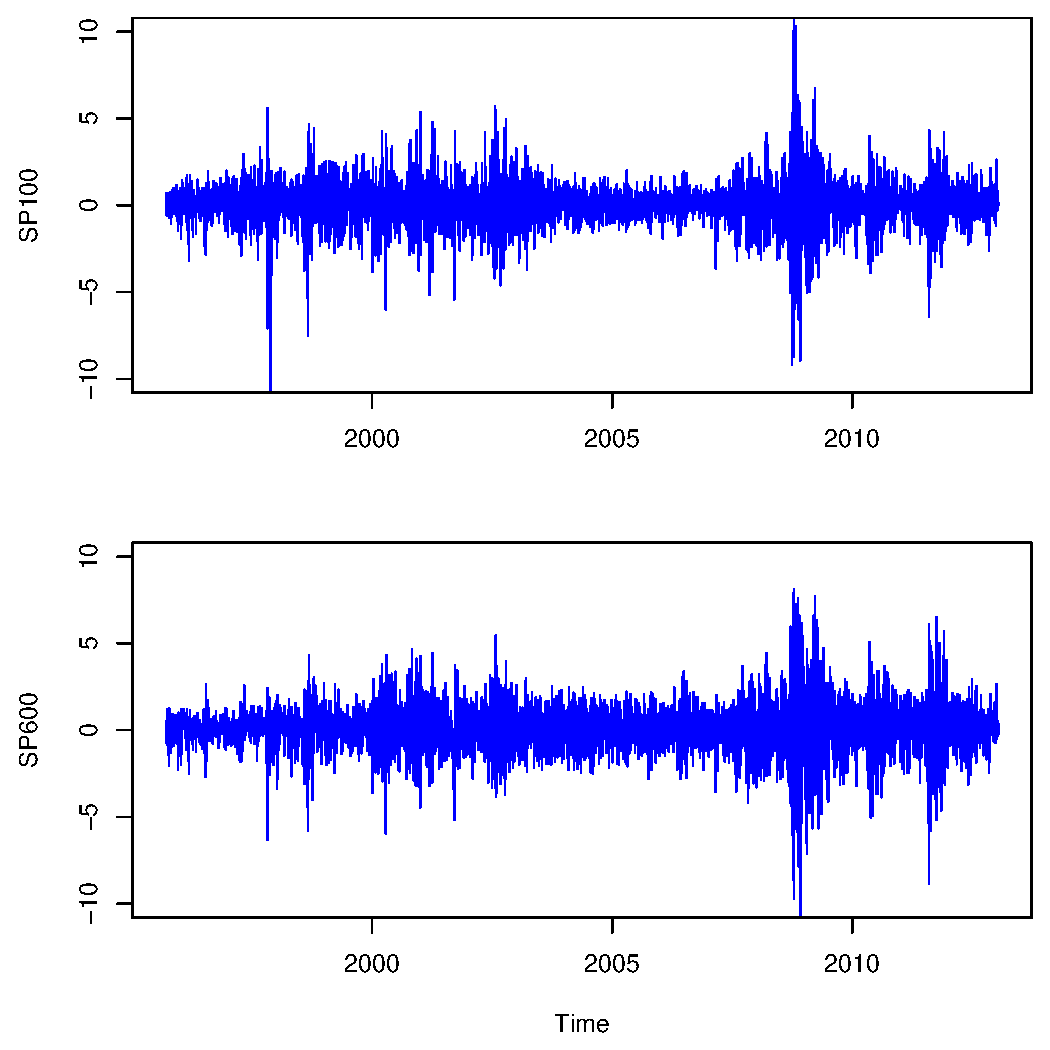
\includegraphics[width=0.6\textwidth]{SP100-SP600}\\
    \includegraphics[width=0.6\textwidth]{SP100-SP600-empCopula}
  \end{figure}
\end{frame}



\begin{frame}
  \frametitle{Covariates in financial data}
  \begin{table}
  \begin{center}
    \caption{Description of covariates used in the model for the S\&P 100 and S\&P 600
      data.}
    \label{tab:sp-covariates}
    \begin{tabular}{lp{0.8\textwidth}l}
      \toprule
      Covariate & Description \\
      \midrule
      \textsf{Return}  & Daily return $y_{t}=100\log(p_{t}/p_{t-1})$ where $p_{t}$ is
                         the closing price. \\
      \textsf{RM1} & Return of last day. \\
      \textsf{RM5} & Return of last week. \\
      \textsf{RM20} & Return of last month. \\
      \textsf{CloseAbs95} & Geometrically decaying average of absolute returns
                            $(1-\rho)\sum\nolimits _{s=0}^{\infty}\rho^{s}|y_{t-2-s}|$
                            with $\rho=0.95$. \\
      \textsf{CloseAbs80} & Geometrically decaying average of past absolute returns
                            with $\rho=0.80$. \\
      \textsf{MaxMin95} & Measure of volatility $(1-\rho)\sum\nolimits
                          _{s=0}^{\infty}\rho^{s}(\log(p_{t-1-s}^{h})-\log(p_{t-1-s}^{l}))$
                          with $\rho=0.95$, where $p^{h}$ and $p^{l}$ are the highest and lowest prices.
      \\
      \textsf{MaxMin80} & Measure of volatility with $\rho=0.80$. \\
      \textsf{CloseSqr95} & Geometrically decaying average of returns
                            $((1-\rho)\sum\nolimits _{s=0}^{\infty}\rho^{s}y_{t-2-s}^{2})^{1/2}$ with
                            $\rho=0.95$. \\
      \textsf{CloseSqr80} & Geometrically decaying average of returns with
                            $\rho=0.80$. \\
      \bottomrule
    \end{tabular}
  \end{center}
\end{table}
\end{frame}


\begin{frame}
  % \frametitle{Improving forecasting performance with covariate-dependent tail-dependence
  %   (Li \& Kang, 2016)}

  \frametitle{Log predictive density score comparison}

\begin{table}
  \begin{center}
    % \caption{Model comparison based on LPS. Note that in principle, the global LPS should
    %   be equal to the summation of LPS values in the marginal and copula components.  But
    %   for numerical reasons in MCMC, they are not exactly the same. The numerical standard
    %   errors are all below one in all LPS values.  }
    % \label{tab:lpds}
    \resizebox{\columnwidth}{!}{%
      \begin{tabular}{llrrrrrrrrrrrrrrr}
        \toprule

        &&\multicolumn{14}{c}{Reparameterized Copulas}\\
        \cline{3-17}
        &&\multicolumn{3}{c}{Joe-Clayton}&&\multicolumn{3}{c}{Clayton}
                                         &&\multicolumn{3}{c}{Gumbel}&&\multicolumn{3}{c}{Student's \emph{t}-Copula}\\
        \cline{3-5} \cline{7-9} \cline{11-13} \cline{15-17}
        &&\multicolumn{1}{c}{\emph{CD.+VS.}}&\multicolumn{1}{c}{\emph{CD.}}
                                         &\multicolumn{1}{c}{\emph{Const.}}&&\multicolumn{1}{c}{\emph{CD.+VS.}}
                                                                     &\multicolumn{1}{c}{\emph{CD.}}&\multicolumn{1}{c}{\emph{Const.}}
                                            &&\multicolumn{1}{c}{\emph{CD.+VS.}}&\multicolumn{1}{c}{\emph{CD.}}
                                                                           &\multicolumn{1}{c}{\emph{Const.}}&&\multicolumn{1}{c}{\emph{CD.+VS.}}
                                                                                                    &\multicolumn{1}{c}{\emph{CD.}}&\multicolumn{1}{c}{\emph{Const.}}\\
        Margins&\multicolumn{1}{c}{LPS}&&&&&&&&&&&&&&&\\

        \midrule

        &&\multicolumn{15}{c}{(\emph{Joint modeling approach})}\\

        SPLIT-\emph{t}&$M_1$
        &$-1743.12$&$-1745.96$&$-1747.99$&&$-1741.04$&$-1805.79$&$-1789.27$&&$-1754.36$
                                                                           &$-1756.09$&$-1756.21$&&$-1741.47$&$-1859.05$&$-1782.37$\\
        &$M_2$
        &$-1435.98$&$-1430.96$&$-1434.22$&&$-1468.25$&$-1589.48$&$-1561.14$&&$-1485.68$
                                                                           &$-1549.39$&$-1563.01$&&$-1430.07$&$-1516.65$&$-1658.09$\\
        &$C$     &$837.50  $&$832.63  $&$779.14  $&&$690.22  $&$774.34  $&$646.57
                                                                           $&&$797.78  $&$794.91  $&$684.60  $&&$792.14  $&$594.60$  &$703.96  $\\
        &$Global$&$-2344.12$&$-2377.01$&$-2411.06$&&$-2523.75$&$-2639.05$&$-2714.69$&&$
                                                                                       -2448.14$&$-2518.48$&$-2639.58$&&$-2380.12$&$-2786.45$&$-2736.49$\\
        \midrule
        &&\multicolumn{15}{c}{(\emph{Two-stage modeling approach})}\\
        SPLIT-\emph{t}&$M_1$
        &$-1740.10$&$-1737.20$&$-1734.57$&&$-1741.05$&$-1735.22$&$-1735.81$&&$-1737.73$
                                                                           &$-1738.03$&$-1736.72$&&$-1741.47$&$-1735.03$&$-1736.18$\\
        &$M_2$
        &$-1428.39$&$-1428.68$&$-1426.78$&&$-1436.63$&$-1425.18$&$-1426.63$&&$-1427.83$
                                                                           &$-1425.19$&$-1428.41$&&$-1433.41$&$-1431.07$&$-1427.53$\\
        &$C$     &$819.63  $&$225.30  $&$121.84  $&&$694.84  $&$262.49  $&$121.50
                                                                           $&&$781.39  $&$621.78  $&$129.60  $&&$788.22  $&$553.50  $&$289.14   $\\
        &$Global$&$-2346.61$&$-2941.80$&$-3045.04$&&$-2483.93$&$-2903.64$&$-3043.71$&&$
                                                                                       -2392.13$&$-2545.14$&$-3036.39$&&$-2389.41$&$-2617.19$&$-2883.14$\\
        \\
        GARCH(1,1)&$M_1$
        &$-1948.07$&$-1948.07$&$-1948.07$&&$-1948.07$&$-1948.07$&$-1948.07$&&$-1948.07$
                                                                           &$-1948.07$&$-1948.07$&&$-1948.07$&$-1948.07$&$-1948.07$\\
        &$M_2$
        &$-1673.85$&$-1673.85$&$-1673.85$&&$-1673.85$&$-1673.85$&$-1673.85$&&$-1673.85$
                                                                           &$-1673.85$&$-1673.85$&&$-1673.85$&$-1673.85$&$-1673.85$\\
        &$C$     &$702.35  $&$495.35  $&$294.18  $&&$530.48  $&$450.42  $&$148.83
                                                                           $&&$810.39  $&$441.49  $&$147.90  $&&$791.55  $&$632.48  $&$598.06  $\\
        &$global$&$-2919.57$&$-3126.56$&$-3327.73$&&$-3091.44$&$-3171.50$&$-3473.09$&&$
                                                                                       -2811.53$&$-3180.43$&$-3474.01$&&$-2830.37$&$-2989.44$&$-3023.86$\\
        \\
        SV        &$M_1$
        &$-2166.90$&$-2159.29$&$-2178.93$&&$-2154.18$&$-2170.90$&$-2194.82$&&$-2168.17$
                                                                           &$-2162.75$&$-2168.62$&&$-2179.36$&$-2186.61$&$-2183.65$\\
        &$M_2$
        &$-1811.36$&$-1809.61$&$-1814.96$&&$-1844.57$&$-1808.54$&$-1787.42$&&$-1808.61$
                                                                           &$-1828.60$&$-1824.77$&&$-1808.24$&$-1830.06$&$-1826.25$\\
        &$C$     &$964.37  $&$768.19  $&$344.22  $&&$698.30  $&$513.081 $&$126.46
                                                                           $&&$1012.10 $&$733.96  $&$231.85 $&&$1053.19 $&$906.58  $&$755.63  $\\
        &$Global$&$-3013.90$&$-3200.70$&$-3649.67$&&$-3300.46$&$-3466.36$&$-3855.78$&&$
                                                                                       -2964.68$&$-3257.39$&$-3761.53$&&$-2934.40$&$-3110.09$&$-3254.27$\\

        \midrule
        &&\multicolumn{15}{c}{(\emph{Bivariate volatility models})}\\

        \multicolumn{2}{l}{Bivariate DCC-GARCH}&$-2730.78$\\
        \multicolumn{2}{l}{Bivariate SV}&$-2999.63$&\\
        \bottomrule
      \end{tabular}
    }
  \end{center}

\end{table}

\end{frame}


\begin{frame}
  \frametitle{}

  \begin{figure}[!h]
    \frametitle{Contour plots of the posterior densities}
    \centering
    \includegraphics[width=0.5\textwidth]{Contour-Post-with-VaR}
  \end{figure}

\end{frame}

\begin{frame}
  \frametitle{Out-of-sample VaR for the portfolio of S\&P 100 and S\&P 600}

  \begin{figure}[h!]
  \centering \includegraphics[width=0.9\textwidth]{VaR001005}
  \caption{The 5\% VaR are calculated for Joe-Clayton copula, Clayton copula, Gumbel
    copula, and bivariate DCC-GARCH models based on 80\% of the historical data. The ratio
    of violations (RoV) indicating the percentage of sample observations lying out of the
    critical values is also reported for each model.}
  \label{fig:VaR-plot}
\end{figure}
\end{frame}





% \section{Detecting credit risk clustering (Li \& He, 2017)}
% \begin{frame}
%   \frametitle{Detecting credit risk clustering (Li \& He,
%     2017)}
%   \framesubtitle{Distance-to-default index}
%   \begin{figure}[!h]
%     \centering
%     \includegraphics[width=0.6\textwidth]{DTD10ts}
%     \caption{Distance-to-default (DTD) for 10 firms. In risk management, the probability of
%       default is high if the value of DTD is small.}
%     \label{fig:DTD-for-ten-firms}
%   \end{figure}

% \end{frame}

% \newcommand{\tabincell}[2]{\begin{tabular}{@{}#1@{}}#2\end{tabular}}
% \begin{frame}
%   \frametitle{Covariates effects on the tail-dependency}
%   \begin{table}
%     % \caption{Covariates effects on the tail-dependency between \textsf{SZKFT} and
%     %   \textsf{CGWC}.}
%   \label{tab:driving-covariates-tail-dependence-coefficients-between-SZKFT-CGWC}
%   \begin{center}
%     \resizebox{0.6\textwidth}{!}{
%     \begin{tabular}{lrrrrrrr}
%       \toprule
%       & \tabincell{l}{No \\ covariates} & & \tabincell{l}{Macroeconomic \\ covariates} & & \tabincell{l}{Specific \\ covariates} & & \tabincell{l}{Macroeconomic and \\ specific covariates} \\
%       \midrule
%       Constant  & $-4.931$  &  & $2.014$ &  & $-2.174$ &  & $10.515$  \\
%       & $(1.000)$ &  & $(1.000)$  &  & $(1.000)$ &  & $(1.000)$  \\
%       CPI       &  &  & $-0.431$  &   &  &  & $-71.814$  \\
%       &  &  & $(0.593)$ &   &  &  &  $(0.507)$  \\
%       M2 growth rate &  &  & $-0.122$  &  &  &  & $2.169$  \\
%       &  &  & $(0.586)$ &  &  &  & $(0.636)$  \\
%       Short-term interest rate &  &  & $-0.012$  &  &  &  & $11.998$  \\
%       &  &  & $(0.988)$ &  &  &  & $(0.254)$  \\
%       RMB/USD spot rate  &  &  & $-0.526$ &  &  &  & $-0.650$  \\
%       &  &  & $(0.605)$  &  &  &  & $(0.309)$  \\
%       \textsf{CGWC}'s solvency capacity  &  &  &  &  & $-0.017$  &  & $4.498$  \\
%       &  &  &  &  & $(0.866)$ &  & $(0.590)$  \\
%       \textsf{CGWC}'s developing capacity   &  &  &  &  & $0.012$   &  & $-1.680$  \\
%       &  &  &  &  & $(0.637)$ &  & $(0.624)$  \\
%       \textsf{CGWC}'s profitability  &  &  &  &  & $0.004$ &  & $-12.948$ \\
%       &  &  &  &  & $(0.751)$  &  & $(0.597)$  \\
%       \textsf{CGWC}'s operating capacity   &  &  &  &  & $-0.039$  &  & $4.819$ \\
%       &  &  &  &  & $(0.716)$ &  & $(0.615)$ \\
%       \textsf{XITG}'s solvency capacity  &  &  &  &  & $0.089$ &  & $58.419$ \\
%       &  &  &  &  & $(0.813)$  &  & $(0.537)$  \\
%       \textsf{XITG}'s developing capacity   &  &  &  &  & $0.030$ &  & $104.257$  \\
%       &  &  &  &  & $(0.652)$ &  & $(0.578)$  \\
%       \textsf{XITG}'s profitability  &  &  &  &  & $-0.409$  &  & $294.978$ \\
%       &  &  &  &  & $(0.531)$ &  & $(0.389)$  \\
%       \textsf{XITG}'s operating capacity   &  &  &  &  & $-0.057$  &  & $-0.305$ \\
%       &  &  &  &  & $(0.857)$ &  & $(0.463)$  \\
%       \midrule
%       LPS  & $-308.732$ &  & $-200.606$ &  & $-106.542$ &  & $-52.831$   \\
%       \bottomrule
%     \end{tabular}
%     }
%   \end{center}
% \end{table}

% \end{frame}

% \section{Multivariate covariate-dependence with mixed margins (Li, Panagiotelis \& Kang, ongoing
%   research)}

% \begin{frame}
%   \frametitle{Multivariate covariate-dependence with mixed margins (Li, Panagiotelis \&
%     Kang, ongoing research)}
%   \framesubtitle{Modeling stock returns and text sentiments}
%   \begin{figure}[!h]
%     \centering
%     % \includegraphics[width=0.55\textwidth]{TextsCovs-New}\\
%     \includegraphics[width=0.27\textwidth]{Alibaba-Stock-Price-R}
%     \includegraphics[width=0.27\textwidth]{Sen-Date-R}
%   \end{figure}



% \end{frame}


% \begin{frame}
%   \frametitle{Covariates in texts data}
%   \begin{figure}
%     \centering
%     \includegraphics[width=0.6\textwidth]{Caixin}\\
%     \includegraphics[width=0.6\textwidth]{TextsCovs-New}
%   \end{figure}
% \end{frame}


% \begin{frame}
%   \frametitle{The dependence between positive/negative sentiments and stocks}

%   \begin{figure}
%     \centering
%     \includegraphics[width=0.45\textwidth]{BABAlambdaLU}
%   \end{figure}

% \end{frame}

\section{Extensions}


\begin{frame}
  \frametitle{Working in progress }

  \begin{itemize}
  \item Modeling multivariate covariate-dependent structure via the vine copula.
  \item Looking into more efficient inference techniques.
  \item Extending to factor (on tail) copula models.
  \end{itemize}
\end{frame}


\begin{frame}[allowframebreaks]
  \frametitle{References}
  \bibliography{References,full}
  \bibliographystyle{asa}
\end{frame}


\begin{frame}[plain]
  \addtocounter{framenumber}{-1}
  \begin{center}
    {\color{SUblue} \textbf{\Huge Thank you!}}
    \vspace{1cm}

    \url{feng.li@cufe.edu.cn}

    \vspace{1cm}

    \url{http://feng.li/}

  \end{center}
\end{frame}

\end{document}
